%%%%%%%%%%%%%%%%%%%%%%%%%%%%%%%%%%%%%%%%%%%%%%%%%%%%%
% REPORT FOR SWISS-SEP 2.0 DATA ANALYSIS
%%%%%%%%%%%%%%%%%%%%%%%%%%%%%%%%%%%%%%%%%%%%%%%%%%%%%

% LATEX settings
\documentclass[a4paper, notitlepage, fleqn]{article} % USE titlepage IF YOU WANT TOC TO APPEAR ON NEXT PAGE
\usepackage[a4paper]{geometry}
\usepackage{stata} 

\usepackage[T1]{fontenc}
\usepackage[utf8]{inputenc}
 
\usepackage{fullpage} % SMALL MARGINS
% \usepackage[cm]{fullpage} % VERY SMALL MARGINS
 
\usepackage{lscape} % BETTER FOR PRINTING, PAGE DISPLAYED VERTICALLY
% \usepackage{pdflscape} % BETTER FOR SCREEN, PAGE DISPLAYED HORIZONTALLY
 
\usepackage{mathtools, amssymb, bookmark, framed, longtable, booktabs, graphicx, url, multirow, cancel}
 
\usepackage{hyperref}
\hypersetup{unicode=true, pdfborder = {0 0 0}, colorlinks, citecolor=blue, filecolor=black, linkcolor=blue, urlcolor=blue, pdftitle={Swiss-SEP 2.0 data analysis}, pdfauthor={Radoslaw Panczak}}

\renewcommand{\familydefault}{\sfdefault}
\usepackage[usenames, dvipsnames]{color}
\usepackage[table]{xcolor}
\usepackage[normalem]{ulem}

\usepackage[hang,flushmargin]{footmisc} 

% to avoid error http://tex.stackexchange.com/questions/165929/semiverbatim-with-tikz-in-beamer
\makeatletter
\global\let\tikz@ensure@dollar@catcode=\relax
\makeatother

\setlength{\parindent}{0pt} % no indent for ne paras
\graphicspath{ {C:/projects/SNC_Swiss-SEP2/analyses/gr} }
\setcounter{tocdepth}{2}

\usepackage{array}
\newcolumntype{L}[1]{>{\raggedright\let\newline\\\arraybackslash\hspace{0pt}}m{#1}}

% \linespread{1.3}
%
% \usepackage{setspace}
% \singlespacing
% \onehalfspacing
% \doublespacing

\usepackage{multirow}

% https://tex.stackexchange.com/questions/52317/pdftex-warning-version-allowed
\pdfminorversion=6

\title{\textbf{Swiss-SEP 2.0 index \endgraf 
Report 1.09 - data analysis}}

\author{Radoslaw Panczak \textit{et al.}}

\begin{document}

\maketitle
\tableofcontents

% %%%%%%%%%%%%%%%%%%%%%%%%%%%%%%%%%%%%%%%%%%%%%%%%%%%%%
% \newpage
% \section{Finding n'hoods with new buildings}
% %%%%%%%%%%%%%%%%%%%%%%%%%%%%%%%%%%%%%%%%%%%%%%%%%%%%%
\newpage
\section{PCA on n'hood aggregated characteristics}
\begin{stlog}\input{log/ol_3.log.tex}\end{stlog}
% %%%%%%%%%%%%%%%%%%%%%%%%%%%%%%%%%%%%%%%%%%%%%%%%%%%%%
\newpage
\section{Building construction period}

Construction period of the building is retrived sfrom \texttt{STATPOP 2018} dataset. Detailed typology is recoded to binary indicator flagging 
buildings constructed on or after 2001. Buidlings with missing information about age are treated as 'old' ones. 
\begin{stlog}\input{log/ol_6.log.tex}\end{stlog}
% %%%%%%%%%%%%%%%%%%%%%%%%%%%%%%%%%%%%%%%%%%%%%%%%%%%%%
\newpage
\section{Hybrid version of SEP}

This solution is mixing versions 1.0 \& 2.0. First the new buildings have value of index 1.0 assigned using the closest (linear dstance) neighbour. 

Then, construction period of the building is retrived sfrom \texttt{STATPOP 2018} dataset and then buildings built before year 2000 have the values of 1.0 index assigned and buildings constructed after 2000 have new values assigned. Buildings without the defined period of construction keep values 1.0 also. 
% %%%%%%%%%%%%%%%%%%%%%%%%%%%%%%%%%%%%%%%%%%%%%%%%%%%%%
\subsection{Index deciles}
\begin{stlog}\input{log/ol_8.log.tex}\end{stlog}
% %%%%%%%%%%%%%%%%%%%%%%%%%%%%%%%%%%%%%%%%%%%%%%%%%%%%%
\subsection{Quantiles}

Note that the deciles of third version in \texttt{full} dataset:
\begin{stlog}\input{log/ol_9.log.tex}\end{stlog}
... are tad 'broken' in \texttt{user} dataset :
\begin{stlog}\input{log/ol_10.log.tex}\end{stlog}
... This is expected behaviour since user dataset excludes buildings with different IDs but same coordinates.  
\begin{landscape}
Some transitions happened:  
\begin{stlog}\input{log/ol_11.log.tex}\end{stlog}
\end{landscape}

% %%%%%%%%%%%%%%%%%%%%%%%%%%%%%%%%%%%%%%%%%%%%%%%%%%%%%
\subsection{Bland Altman plots of diffs}
\subsubsection{SEP2 vs. SEP1}

\begin{center}
\includegraphics[width=\textwidth]{gr/BA_sep1_sep2.png} 
\end{center}

\subsubsection{SEP3 vs. SEP1}

\begin{center}
\includegraphics[width=\textwidth]{gr/BA_sep1_sep3.png} 
\end{center}
% %%%%%%%%%%%%%%%%%%%%%%%%%%%%%%%%%%%%%%%%%%%%%%%%%%%%%
\newpage
\section{Tables}

\newpage
\subsection{Old index}
\begin{landscape}
\begin{footnotesize}
\input(table-1)
\end{footnotesize}
\end{landscape}

\newpage
\subsection{New index}
\begin{landscape}
\begin{footnotesize}
\input(table-2)
\end{footnotesize}
\end{landscape}

\newpage
\subsection{Hybrid index}
\begin{landscape}
\begin{footnotesize}
\input(table-3")
\end{footnotesize}
\end{landscape}

% %%%%%%%%%%%%%%%%%%%%%%%%%%%%%%%%%%%%%%%%%%%%%%%%%%%%%
\newpage
\section{Maps}
\subsection{Original map}

\begin{center}
\includegraphics[width=\textwidth]{gr/sep-old.png} 
\end{center}

\newpage 
\subsection{SEP 2 \& 3 index}

Using hexagonal grid 500m size.  

\begin{center}
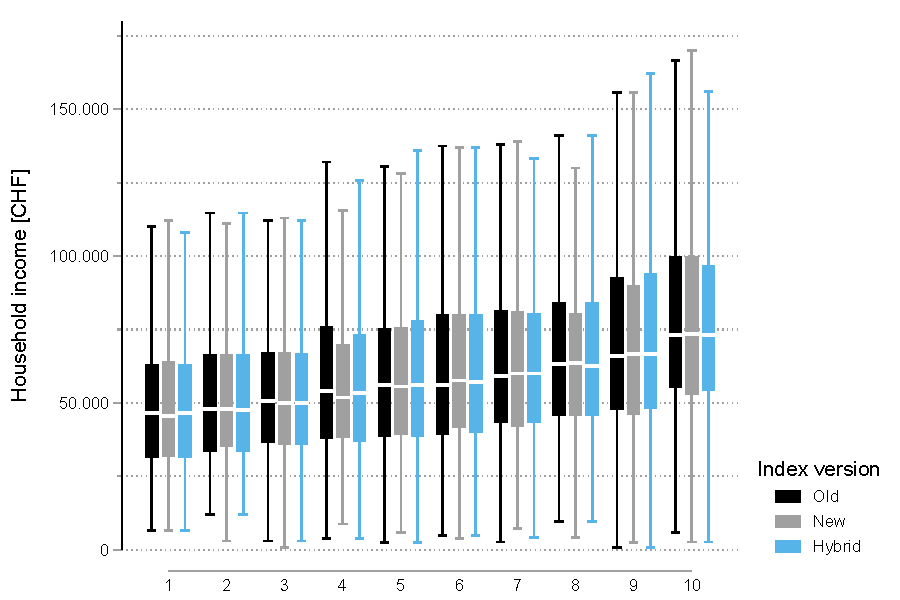
\includegraphics[width=\textwidth]{C:/projects/SNC_Swiss-SEP2/analyses/Figure_1.png} 
\end{center}

\newpage
\subsection{Differences}

\begin{center}
\includegraphics[width=\textwidth]{C:/projects/SNC_Swiss-SEP2/carto/08_sep-diff-grid_hex_500.png} 
\end{center}

% %%%%%%%%%%%%%%%%%%%%%%%%%%%%%%%%%%%%%%%%%%%%%%%%%%%%%
% %%%%%%%%%%%%%%%%%%%%%%%%%%%%%%%%%%%%%%%%%%%%%%%%%%%%%
\newpage
\section{Validation - SHP data}

% %%%%%%%%%%%%%%%%%%%%%%%%%%%%%%%%%%%%%%%%%%%%%%%%%%%%%
\subsection{Income graph - original}

\begin{center}
\includegraphics[width=.75\textwidth]{gr-orig/orig_income.png} 
\end{center}

% %%%%%%%%%%%%%%%%%%%%%%%%%%%%%%%%%%%%%%%%%%%%%%%%%%%%%
\subsection{Income graph - new indices}
\begin{center}
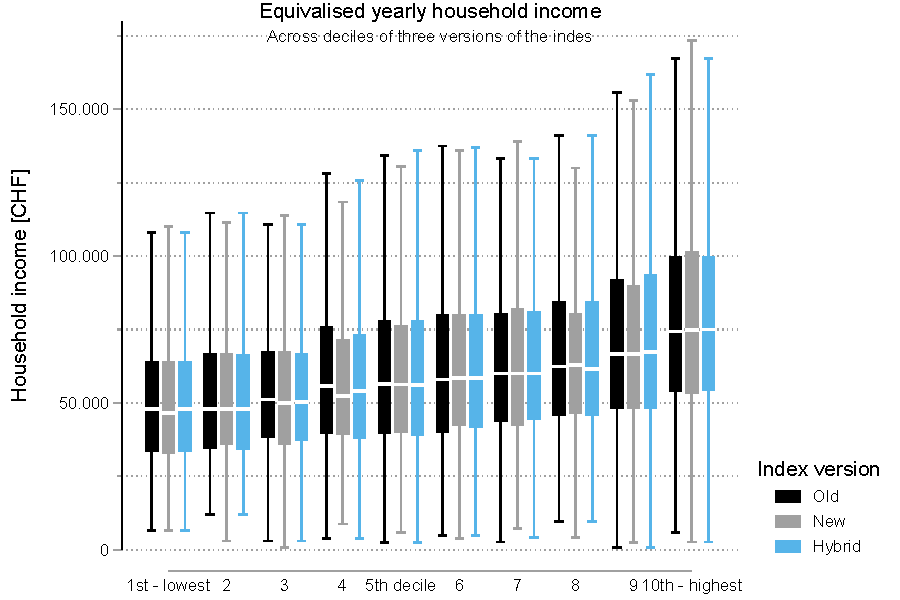
\includegraphics[width=.75\textwidth]{gr/shp_income.pdf} 
\end{center}

% %%%%%%%%%%%%%%%%%%%%%%%%%%%%%%%%%%%%%%%%%%%%%%%%%%%%%
\newpage
\subsection{Financial variables table - original}

\begin{center}
\includegraphics[width=.95\textwidth]{gr-orig/orig_shp_table.png} 
\end{center}

% %%%%%%%%%%%%%%%%%%%%%%%%%%%%%%%%%%%%%%%%%%%%%%%%%%%%%
\newpage
\subsection{Financial variables table - 1.0}
\begin{stlog}\input{log/ol_14.log.tex}\end{stlog}
\newpage
\begin{stlog}\input{log/ol_15.log.tex}\end{stlog}
\newpage
\begin{stlog}\input{log/ol_16.log.tex}\end{stlog}
% %%%%%%%%%%%%%%%%%%%%%%%%%%%%%%%%%%%%%%%%%%%%%%%%%%%%%
\newpage
\subsection{Financial variables table - 2.0}
\begin{stlog}\input{log/ol_17.log.tex}\end{stlog}
\newpage
\begin{stlog}\input{log/ol_18.log.tex}\end{stlog}
\newpage
\begin{stlog}\input{log/ol_19.log.tex}\end{stlog}
% %%%%%%%%%%%%%%%%%%%%%%%%%%%%%%%%%%%%%%%%%%%%%%%%%%%%%
\newpage
\subsection{Financial variables table - 3.0}
\begin{stlog}\input{log/ol_20.log.tex}\end{stlog}
\newpage
\begin{stlog}\input{log/ol_21.log.tex}\end{stlog}
\newpage
\begin{stlog}\input{log/ol_22.log.tex}\end{stlog}
% %%%%%%%%%%%%%%%%%%%%%%%%%%%%%%%%%%%%%%%%%%%%%%%%%%%%%
\newpage
\section{Validation - SNC mortality}

\subsection{All cause mortality - original}

\begin{center}
\includegraphics[width=.50\textwidth, angle = 270]{gr-orig/orig_hr_all.png} 
\end{center}

Note: 	Calculations from 'old' SNC data from the \textbf{2001 - 2008 period}, as described in original paper!

% %%%%%%%%%%%%%%%%%%%%%%%%%%%%%%%%%%%%%%%%%%%%%%%%%%%%%
\subsection{All cause mortality - new indices}
\begin{center}
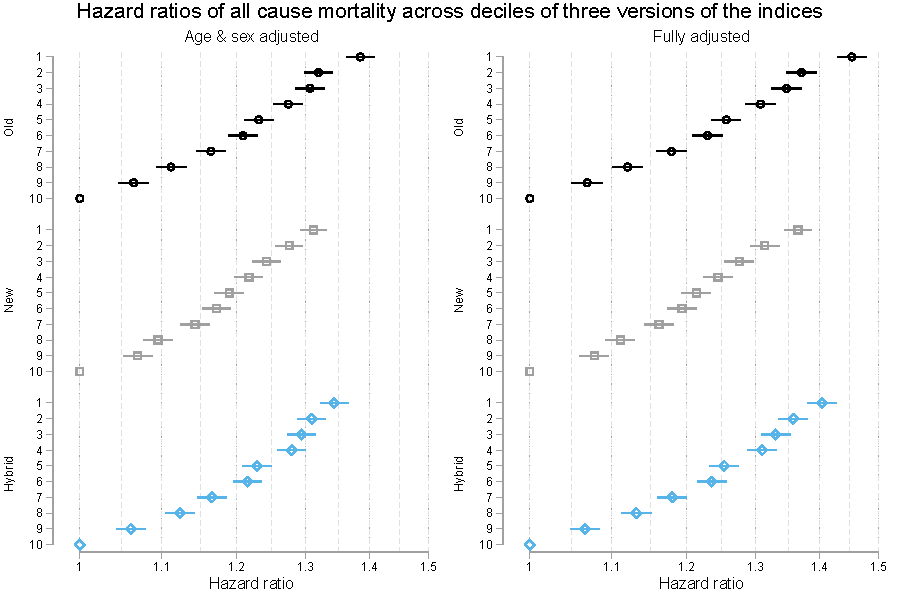
\includegraphics[width=\textwidth]{gr/sep3.pdf}
\end{center}

Note: 	Results from Cox models. Calculations from 'new' SNC data from the \textbf{2012 - 2018 period}!  
		'Age \& sex' - adjusted for age (via \texttt{stset}) and sex (as in original figure above);  
		'Adjusted' - additionally adjusted for civil status, nationality, level of urbanization and language region.  
		This is not the same adjustment as in adsjudsted models in original papers since we are missing some crucial variables. 
% %%%%%%%%%%%%%%%%%%%%%%%%%%%%%%%%%%%%%%%%%%%%%%%%%%%%%
\newpage
\subsection{Cause specific mortality - original}

\begin{center}
\includegraphics[width=.60\textwidth]{gr-orig/orig_hr_spec.png} 
\end{center}

% %%%%%%%%%%%%%%%%%%%%%%%%%%%%%%%%%%%%%%%%%%%%%%%%%%%%%
\newpage
\subsection{Cause specific mortality - 1.0}
\begin{stlog}\input{log/ol_25.log.tex}\end{stlog}
Note for both tables: HRs for the 10th (lowest SEP) decile compared to 1st (highest SEP). 
Breast and prostate cancer: for men and women respectively. 

% %%%%%%%%%%%%%%%%%%%%%%%%%%%%%%%%%%%%%%%%%%%%%%%%%%%%%
\newpage
\subsection{Cause specific mortality - 2.0 results}
\begin{stlog}\input{log/ol_27.log.tex}\end{stlog}
Note for both tables: HRs for the 10th (lowest SEP) decile compared to 1st (highest SEP). 
Breast and prostate cancer: for men and women respectively. 

% %%%%%%%%%%%%%%%%%%%%%%%%%%%%%%%%%%%%%%%%%%%%%%%%%%%%%
\newpage
\subsection{Cause specific mortality - 3.0 results}
\begin{stlog}\input{log/ol_29.log.tex}\end{stlog}
Note for both tables: HRs for the 10th (lowest SEP) decile compared to 1st (highest SEP). 
Breast and prostate cancer: for men and women respectively. 
\end{document}
